% 请在下方的大括号相应位置填写正确的节标题和标签,以及作者姓名
\section{磁矩计算}\label{sec:磁矩计算}
\sectionAuthor{Jiaqi Z.}

% 请在下方的item内填写本节知识点
\begin{Abstract}
    \item 如何计算体系磁矩
    \item 如何根据能量确定磁基态
    \item 如何查看磁矩分布
    \item 绘制自旋密度图
\end{Abstract}

这一节,我们将介绍如何计算磁性材料,主要考察它们的磁性,以及磁矩分布等问题。结合前面的能量计算,我们还有可能接触到一点关于铁磁和反铁磁的性质讨论。

\subsection{计算体系磁矩\code{ISPIN=2}}\label{subsec:磁矩计算-计算体系磁矩ISPIN=2}

下面这个例子,计算了一个单原子Si的磁矩。之所以先计算单原子,是因为单原子的磁矩比较容易分析。首先,我们先构建只有一个Si原子的\code{POSCAR}

\begin{lstlisting}[caption=POSCAR]
Si
1.0
    5.0 0.0 0.0
    0.0 5.0 0.0
    0.0 0.0 5.0
Si    
1
Direct
0.5 0.5 0.5
\end{lstlisting}

接下来构建\code{INCAR}文件

\begin{lstlisting}[caption=INCAR]
ISTART =  1
ISPIN  =  2
LREAL  = .FALSE.
ENCUT  =  600
LWAVE  = .FALSE.
LCHARG = .FALSE.
ADDGRID= .TRUE.
LASPH  = .TRUE.
PREC   = Accurate
ISMEAR =  0
SIGMA  =  0.05
NELM   =  60
EDIFF  =  1E-5
\end{lstlisting}

这个参数与\ref{sec:能量计算}一节所使用的几乎完全相同,唯一有一个不同的地方是\keywordin{INCAR}{ISPIN}设置为2,表示\emph{开启自旋极化}。此外,由于我们是计算单原子(不考虑重复单元),与计算分子类似,使用$1\times1\times1$的\code{KPOINTS}。

\begin{attention}
    由于是计算单原子,因此也不存在结构优化这回事。毕竟一个原子无论从晶格还是坐标都没有可优化的地方(哪怕分数坐标从0.5变成0.6也没有任何意义)。

    这件事与计算分子不同,分子需要进行坐标优化(涉及到键长),也就是\ref{sec:对坐标进行优化ISIF=2}一节所介绍的例子。
\end{attention}

当计算完成后,我们考察\code{OSZICAR}文件,与\code{ISPIN=1}不同的地方在于,每一个离子步后面多了一个\code{mag}表示体系磁矩。\emph{关注最后一行的\code{mag}},其数值就表示体系的磁矩。在本例中,最后一行的\code{OSZICAR}如下所示:

\begin{lstlisting}[caption=OSZICAR]
1 F= -.44168179E+00 E0= -.42239900E+00  d E =-.385656E-01  mag=     2.0000
\end{lstlisting}

表示体系的磁矩为2.0,单位为玻尔磁子$\mu_\text{B}$,这一结论与Si原子的电子排布结论相同\footnote{正如原子物理或者高中化学所介绍的那样,Si有两个3p孤立电子,从而表现为磁矩为2.0 $\mu_\text{B}$}。但是,如果我们考察一下VASP计算得到的电子占据(无论从\keyword{EIGENVAL}文件读取还是从\code{OUTCAR}最后查看不同能量的电子排布),都会发现类似下面的情况(我们这里以\code{OUTCAR}为例):

\begin{lstlisting}[caption=OUTCAR]
spin component 1

k-point     1 :       0.0000    0.0000    0.0000
band No.  band energies     occupation
    1      -9.4957      1.00000
    2      -2.2461      0.66667
    3      -2.2461      0.66667
    4      -2.2461      0.66667
    5       0.7529      0.00000
    6       3.1135      0.00000
    7       3.1135      0.00000
(略一部分)
spin component 2

k-point     1 :       0.0000    0.0000    0.0000
band No.  band energies     occupation
    1      -7.7339      1.00000
    2      -0.4696      0.00000
    3      -0.4696      0.00000
    4      -0.4696      0.00000
    5       1.5279      0.00000
    6       4.1230      0.00000
(下略)
\end{lstlisting}

可以看到,对于spin为1的状态,电子占据数出现了0.66667这样的小数,这显然是不合理的。之所以出现这个结果,是因为在计算时出现了“简并”,即出现了三个能量是-2.2461的轨道,且由这三个轨道均分两个电子,从而每个轨道分得0.66667(也就是三分之二)个电子。

\begin{attention}
    在这里我们说\emph{spin为1的状态},并没有特指自旋向上或向下。事实上,自旋方向是人为定义的,你可以说spin为1是自旋向上,也可以说它是自旋向下。

    在本教程中,若无特殊说明,我们默认spin为1表示自旋向上,磁矩为正表示自旋向上。
\end{attention}

之所以产生这个问题,一个原因是\emph{我们所使用的晶格常数对称性太高了}。如果我们想办法减小一点对称性,将\code{POSCAR}中的晶格常数改为5.0 5.5 5.9,再次进行计算,结果在保持磁矩为2.0不变的前提下,电子占据也会变得正常:

\begin{lstlisting}[caption=OUTCAR]
spin component 1

k-point     1 :       0.0000    0.0000    0.0000
band No.  band energies     occupation
    1     -10.0597      1.00000
    2      -3.3334      1.00000
    3      -3.1172      1.00000
    4      -2.6324      0.00000
    5      -0.0094      0.00000
    6       2.0529      0.00000
    7       2.6188      0.00000

(略一部分)
spin component 2

k-point     1 :       0.0000    0.0000    0.0000
band No.  band energies     occupation
    1      -8.5155      1.00000
    2      -1.9085      0.00000
    3      -1.3910      0.00000
    4      -1.0711      0.00000
    5       0.6883      0.00000
    6       2.8908      0.00000
(下略)
\end{lstlisting}

此时自旋向上有3个电子,自旋向下有1个电子,与实际排布情况相同\footnote{我们这里讨论的是价电子,具体的电子排布式写作[Ne]3s$^2$3p$^2$}。

\subsection{使用\code{MAGMOM}设置初始磁矩}\label{subsec:磁矩计算-使用MAGMOM设置初始磁矩}

下面我们将进一步讨论多原子体系,讨论两个Cr原子组成的体系,其\code{POSCAR}如下所示\footnote{你可以在Materials Project里下载这个结构:https://next-gen.materialsproject.org/materials/mp-90}:

\begin{lstlisting}[caption=POSCAR]
Cr2
1.0
    2.9688993551160281    0.0000000000000000    0.0000000000000002
    -0.0000000000000002    2.9688993551160281    0.0000000000000002
    0.0000000000000000    0.0000000000000000    2.9688993551160281
Cr
2
direct
    0.0000000000000000    0.0000000000000000    0.0000000000000000 Cr0+
    0.5000000000000000    0.5000000000000000    0.5000000000000000 Cr0+
\end{lstlisting}

与单原子不同的地方在于,首先需要对体系进行结构优化(使用\code{ISIF=3})。但与\ref{sec:对晶格常数进行优化ISIF=3}不同的地方在于,对磁性材料进行结构优化时也应当开启\code{ISPIN=2}。

\begin{attention}
    自旋极化打开与否是会影响体系结构的,甚至不同的磁性都有可能产生不同的结构。
\end{attention}

完成后进行静态自洽计算,与前面的讨论接近,使用如下的\code{INCAR}:

\begin{lstlisting}[caption=INCAR]
ISTART =  1
ISPIN  =  2
LREAL  = .FALSE.
ENCUT  =  450
LWAVE  = .FALSE.
LCHARG = .FALSE.
ADDGRID= .TRUE.
LASPH  = .TRUE.
PREC   = Accurate
ISMEAR =  0
SIGMA  =  0.05
LORBIT =  11
NELM   =  60
EDIFF  =  1E-5
\end{lstlisting}

有一点不同的地方,在于设置了\keywordin{INCAR}{LORBIT}参数。当\code{LORBIT=10}时表示将轨道投影到$s,p,d$,而\code{LORBIT=11}则可以进一步将轨道投影至如$p_x,p_y,p_z$等。在本例中,使用\code{LORBIT=10}或\code{LORBIT=11}均不影响结果。

计算完成后,查看\code{OSZICAR},发现体系磁矩为0,表示体系没有磁性。当设置\code{LORBIT}之后,我们可以通过\code{OUTCAR}查看每个原子的磁矩。在接近最后的位置,可以有如下输出内容:

\begin{lstlisting}[caption=OUTCAR]
magnetization (x)

# of ion       s       p       d       tot
------------------------------------------
    1        0.000  -0.000  -0.000  -0.000
    2        0.000  -0.000  -0.000  -0.000
--------------------------------------------------
tot          0.000  -0.000  -0.000  -0.000
\end{lstlisting}

其中原子编号是按照\code{POSCAR}顺序,里面的\code{tot}一列表示原子的总磁矩(沿$z$轴方向),可以发现,每个原子的磁矩都为0.

\begin{extend}
    我们这里所说是沿着$z$轴方向的磁矩,但实际计算时当然可以指定具体方向,具体来说,这个过程涉及到非共线计算(\keywordin{INCAR}{LNONCOLLINEAR}设置为\code{.TRUE.},同时设置\keywordin{INCAR}{LSORBIT}为\code{.TRUE.}开启自旋轨道耦合(Spin-orbit coupling, SOC),并在\keywordin{INCAR}{SAXIS}里设置量化轴方向。

    此外,在计算SOC时,还应当使用非共线版本的vasp(目前默认使用的都是vasp\_std),需要将“std”改为“ncl”。
\end{extend}

但是,事实真的如此吗?如果是从Materials Project下载的数据,可以看一下上面对磁性的描述,是\emph{Antiferromagnetic},也就是\emph{反铁磁}。所谓“反铁磁”,指的是“在没有外部磁场的情况下,材料内部相邻原子的磁矩相互抵消,形成反平行排列的状态。这种排列使得材料在宏观上不表现出磁性,即净磁矩为零”。但是,我们如何想办法得到这个反铁磁态呢?就需要在计算时设置\keywordin{INCAR}{MAGMOM}参数给定初始磁矩。

在这里,我们假定每个原子的磁矩是6,这是我们已知的原子磁矩。在原先的\code{INCAR}中添加\code{MAGMOM = 9 9}表示\emph{设置第一个原子的磁矩为9,第二个原子的磁矩为9}。

在设置\code{MAGMOM}时,你可以像这里这样直接给出每个原子的磁矩(按照\code{POSCAR}顺序),如果原子数较多,也可以使用\code{*}批量设置,其格式为\code{[number]*[mag]},其\emph{符号前后没有空格},但每一组之间用空格分隔。例如,\code{MAGMOM=16*0 1*2}表示前十六个原子磁矩为0,后一个原子磁矩为2.

\begin{attention}
    在这里我们设置的磁矩是初始磁矩,VASP会有方法将其收敛到合适的值。通常来说,我们要给的初始值应当比真实值大,在这里我们设置为9,当然设置为其他数值也是可以的。但不同的初始值可能会计算到不同的磁矩。

    此外,正如前面所说的那样,不同的磁矩会影响不同的结构,因此在设置\code{MAGMOM}时需要从结构优化开始。
\end{attention}

无论你是怎样设置的磁矩,在计算后得到的磁矩与上面的\code{OUTCAR}接近。查看体系的能量,发现约为-19.03 eV。如果我们尝试设置为反铁磁态(即两个原子的磁矩相反),例如,设置\code{MAGMOM=-9 9},重复上面的结构优化与自洽计算,会发现能量为-19.06 eV,比前面的能量更低。这一结论表明\emph{后面的状态为更稳定的基态}(有时也管这种状态叫\emph{磁基态})。当我们进一步考察其\code{OUTCAR}时,可以发现结果为:

\begin{lstlisting}[caption=OUTCAR]
magnetization (x)

# of ion       s       p       d       tot
------------------------------------------
    1       -0.014  -0.008  -1.078  -1.100
    2        0.014   0.008   1.078   1.100
--------------------------------------------------
tot          0.000   0.000   0.000   0.000 
\end{lstlisting}

其中\emph{第一个原子和第二个原子磁矩大小相同,方向相反,总磁矩表现为0}(在\code{OSZICAR}中可以查看),这种状态就是\emph{反铁磁}。

\begin{attention}
    我们在这里只讨论\code{MAGMOM=9 9}和\code{MAGMOM=-9 9}的情况,对于另外两种情况(-9 -9和9 -9),其本质与前面两种相同。正如前面所说的,自旋方向是相对的,两个都自旋向上,与两个都自旋向下,结果是一样的。
\end{attention}

\begin{extend}
    我们在这里介绍了\code{MAGMOM}的两种设置方法,除此之外还有第三种,即设置原子沿每个轴的磁矩。这一设置需要使用前面所介绍的“非共线计算”(\code{LNONCOLLINEAR=.TRUE.})。这里暂不介绍,如有需要,可查看VASP对\code{MAGMOM}的介绍\footnote{https://vasp.at/wiki/MAGMOM}。
\end{extend}

\subsection{自旋密度图可视化}\label{subsec:磁矩计算-自旋密度图可视化}

在前面的计算中,我们已经找到了Cr的磁矩分布,但在论文中,有时为了强调磁矩的分布情况(如具体是哪个原子提供磁矩,磁矩方向如何等),我们会考虑绘制\emph{自旋密度图}。具体的计算方法与上面所讨论的类似,但唯一需要修改的一个参数是\code{LCHARG=.TRUE.}生成\code{CHGCAR}文件。具体来说,下面是一个完整的自洽计算的\code{INCAR}例子:

\begin{lstlisting}[caption=INCAR]
ISTART =  1
ISPIN  =  2
MAGMOM =  -9 9
LREAL  = .FALSE.
ENCUT  =  450
LWAVE  = .FALSE.
LCHARG = .TRUE.
ADDGRID= .TRUE.
LASPH  = .TRUE.
PREC   = Accurate
ISMEAR =  0
SIGMA  =  0.05
LORBIT =  11
NELM   =  60
EDIFF  =  1E-5
\end{lstlisting}

具体的绘制方法,使用\code{vaspkit-312}的“Spin Density”功能处理,之后生成\code{SPIN.vasp}文件,将其拖动到可视化软件\code{VESTA}当中,稍微调整一下等值面(在“Properties”-“Isosurfaces”当中),这里设置为0.01,如图\ref{fig:磁矩计算-Cr自旋密度图}所示:

\begin{figure}
    \centering
    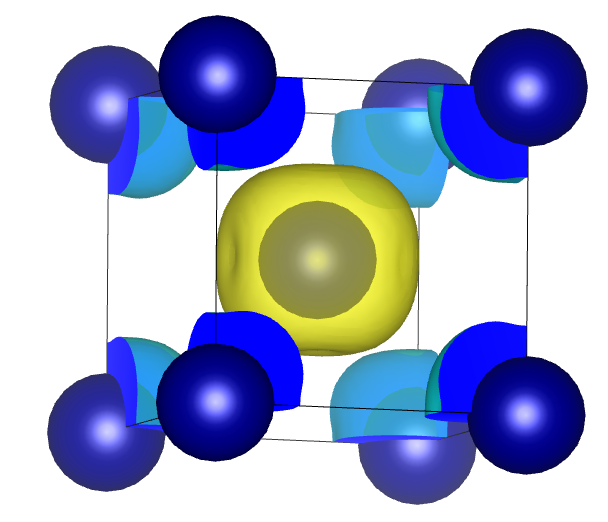
\includegraphics[width=1\linewidth]{VASP计算/静态自洽与电荷密度/磁矩计算/fig/Cr自旋密度图.png}
    \caption{Cr自旋密度图}
    \label{fig:磁矩计算-Cr自旋密度图}
\end{figure}

可以发现,中间的原子与角上的原子自旋方向不同,与我们的结论一致。


% \subsection{错误处理}\label{subsec:节标题-错误处理}
% % 请在本节列出可能遇见的错误与解决方法

% \subsubsection{错误1}

% \subsubsection{错误2}

% \subsubsection{错误3}